\documentclass[11pt,]{article}
\usepackage[]{mathpazo}
\usepackage{amssymb,amsmath}
\usepackage{ifxetex,ifluatex}
\usepackage{fixltx2e} % provides \textsubscript
\ifnum 0\ifxetex 1\fi\ifluatex 1\fi=0 % if pdftex
  \usepackage[T1]{fontenc}
  \usepackage[utf8]{inputenc}
\else % if luatex or xelatex
  \ifxetex
    \usepackage{mathspec}
  \else
    \usepackage{fontspec}
  \fi
  \defaultfontfeatures{Ligatures=TeX,Scale=MatchLowercase}
\fi
% use upquote if available, for straight quotes in verbatim environments
\IfFileExists{upquote.sty}{\usepackage{upquote}}{}
% use microtype if available
\IfFileExists{microtype.sty}{%
\usepackage{microtype}
\UseMicrotypeSet[protrusion]{basicmath} % disable protrusion for tt fonts
}{}
\usepackage{hyperref}
\PassOptionsToPackage{usenames,dvipsnames}{color} % color is loaded by hyperref
\hypersetup{unicode=true,
            colorlinks=true,
            linkcolor=black,
            citecolor=black,
            urlcolor=black,
            breaklinks=true}
\urlstyle{same}  % don't use monospace font for urls
\usepackage{natbib}
\bibliographystyle{amnat}
\usepackage{graphicx,grffile}
\makeatletter
\def\maxwidth{\ifdim\Gin@nat@width>\linewidth\linewidth\else\Gin@nat@width\fi}
\def\maxheight{\ifdim\Gin@nat@height>\textheight\textheight\else\Gin@nat@height\fi}
\makeatother
% Scale images if necessary, so that they will not overflow the page
% margins by default, and it is still possible to overwrite the defaults
% using explicit options in \includegraphics[width, height, ...]{}
\setkeys{Gin}{width=\maxwidth,height=\maxheight,keepaspectratio}
\IfFileExists{parskip.sty}{%
\usepackage{parskip}
}{% else
\setlength{\parindent}{0pt}
\setlength{\parskip}{6pt plus 2pt minus 1pt}
}
\setlength{\emergencystretch}{3em}  % prevent overfull lines
\providecommand{\tightlist}{%
  \setlength{\itemsep}{0pt}\setlength{\parskip}{0pt}}
\setcounter{secnumdepth}{0}
% Redefines (sub)paragraphs to behave more like sections
\ifx\paragraph\undefined\else
\let\oldparagraph\paragraph
\renewcommand{\paragraph}[1]{\oldparagraph{#1}\mbox{}}
\fi
\ifx\subparagraph\undefined\else
\let\oldsubparagraph\subparagraph
\renewcommand{\subparagraph}[1]{\oldsubparagraph{#1}\mbox{}}
\fi

%%% Use protect on footnotes to avoid problems with footnotes in titles
\let\rmarkdownfootnote\footnote%
\def\footnote{\protect\rmarkdownfootnote}

%%% Change title format to be more compact
\usepackage{titling}

% Create subtitle command for use in maketitle
\providecommand{\subtitle}[1]{
  \posttitle{
    \begin{center}\large#1\end{center}
    }
}

\setlength{\droptitle}{-2em}

  \title{}
    \pretitle{\vspace{\droptitle}}
  \posttitle{}
    \author{}
    \preauthor{}\postauthor{}
    \date{}
    \predate{}\postdate{}
  
%%% Modified from Latex Template for Am. Nat., many other details aren't necessary because they are specified in YAML header of Rmarkdown document.
\usepackage{fullpage}
\linespread{1.7}
\usepackage{lineno}

% code below is important for holding figure positions in main text. Make sure to set fig.pos="H" in code chunk for figure.
\usepackage{float}
\let\origfigure\figure
\let\endorigfigure\endfigure
\renewenvironment{figure}[1][2] {
    \expandafter\origfigure\expandafter[H]
} {
    \endorigfigure
}

\begin{document}

\vspace*{0.1cm}

\begin{center} \LARGE Supplementary Material: \\
Loss of consumers constrains phenotypic evolution in the resulting food web \end{center}

\bigskip

\begin{center} \large Matthew A. Barbour$^{1,2,\ast}$, Christopher J. Greyson-Gaito$^{2,3}$, Arezoo Sootodeh$^{2}$, Brendan Locke$^{4}$, Jordi Bascompte$^{1}$ \normalsize \end{center}

\bigskip

\noindent 1. University of Zurich, Department of Evolutionary Biology
and Environmental Studies, Zurich, 8057 ZH, Switzerland;

\noindent 2. University of British Columbia, Department of Zoology,
Vancouver, BC V6T 1Z4, Canada;

\noindent 3. University of Guelph, Department of Integrative Biology,
Guelph, ON N1G 2W1, Canada;

\noindent 4. Humboldt State University, Department of Biological
Sciences, Arcata, CA 95521, USA.

\(^\ast\) Corresponding author; e-mail:
\href{mailto:matthew.barbour@ieu.uzh.ch}{\nolinkurl{matthew.barbour@ieu.uzh.ch}}

\linenumbers{} \modulolinenumbers[3]

\newcommand{\beginsupplement}{%
        \setcounter{table}{0}
        \renewcommand{\thetable}{S\arabic{table}}%
        \setcounter{figure}{0}
        \renewcommand{\thefigure}{S\arabic{figure}}%
     }

\newpage

\beginsupplement

\begin{table}[h]
\caption{Standardized selection gradients acting on egg parasitoids (\textit{Platygaster} sp.)}
\label{Table:ExtendedGradients}
\centering
\begin{tabular}{lc}
\\ 
\hline
\textbf{Selection gradient} & \textbf{Contrast = Original - Removal}  \\ 
\hline
$\beta_{\text{Diam}}$ & 

-0.03 [
-0.3,
0.25] \\

$\beta_{\text{Clutch}}$ & 

0.07 [
-0.26,
0.39] \\

$\beta_{\text{Pref}}$ &

-0.25 [
-0.64,
0.09] \\

$\gamma_{\text{Diam:Diam}}$ &

-0.05 [
-0.43,
0.33] \\

$\gamma_{\text{Clutch:Clutch}}$ & 

-0.21 [
-0.68,
0.26] \\

$\gamma_{\text{Pref:Pref}}$ & 

\textbf{
-0.46 [
-1.07,
-0.02] }\\

$\gamma_{\text{Diam:Clutch}}$ & 

0 [
-0.29,
0.27] \\

$\gamma_{\text{Diam:Pref}}$ & 

0.25 [
-0.04,
0.6] \\

$\gamma_{\text{Clutch:Pref}}$ & 

-0.18 [
-0.52,
0.12] \\ 
\hline
\end{tabular}
\bigskip{}
\\
{\footnotesize Note: Values in brackets represent 95\% confidence intervals. Bold values indicate that the 95\% CI does not overlap zero. $\beta_{\text{Diam}}$ has been adjusted for bias.}
\end{table}

\newpage

\begin{table}[h]
\caption{Standardized selection gradients imposed by larval parasitoids on gall midges in the original food web. This gives insight to selection acting on gall midges in the absence of the dominant egg parasitoid.}
\label{Table:LarvalGradients}
\centering
\begin{tabular}{lc}
\\ 
\hline
\textbf{Selection gradient} & \textbf{Larval Parasitoids} \\ % & \textbf{Original} 
\hline
$\beta_{\text{Diam}}$ & 
%\textbf{
%0.34 [
%0.22,
%0.48] } & 
\textbf{
0.23 [
0.13,
0.36] } \\

$\beta_{\text{Clutch}}$ & 
%0.06 [
%-0.05,
%0.17] & 
\textbf{
0.13 [
0.04,
0.24] }\\

$\beta_{\text{Pref}}$ &
%-0.13 [
%-0.29,
%0.05] & 
\textbf{
-0.17 [
-0.34,
-0.03] } \\

$\gamma_{\text{Diam:Diam}}$ &
%0.13 [
%-0.06,
%0.33] & 

0.06 [
-0.07,
0.2]  \\

$\gamma_{\text{Clutch:Clutch}}$ & 
%-0.05 [
%-0.27,
%0.18] & 

0.01 [
-0.14,
0.15] \\

$\gamma_{\text{Pref:Pref}}$ & 
%\textbf{
%0.34 [
%0.07,
%0.63] }& 

0.18 [
-0.02,
0.42] \\

$\gamma_{\text{Diam:Clutch}}$ & 
%-0.04 [
%-0.16,
%0.08] & 

0.02 [
-0.07,
0.11]  \\

$\gamma_{\text{Diam:Pref}}$ & 
%-0.13 [
%-0.29,
%0.02] & 

-0.05 [
-0.18,
0.06]  \\

$\gamma_{\text{Clutch:Pref}}$ & 
%0.03 [
%-0.1,
%0.18] & 

-0.04 [
-0.14,
0.06]  \\ 
\hline
\end{tabular}
\bigskip{}
\\
{\footnotesize Note: Values in brackets represent 95\% confidence intervals. Bold values indicate that the 95\% CI does not overlap zero. $\beta_{\text{Diam}}$ has been adjusted for bias.}
\end{table}

\newpage

\begin{figure}
\centering
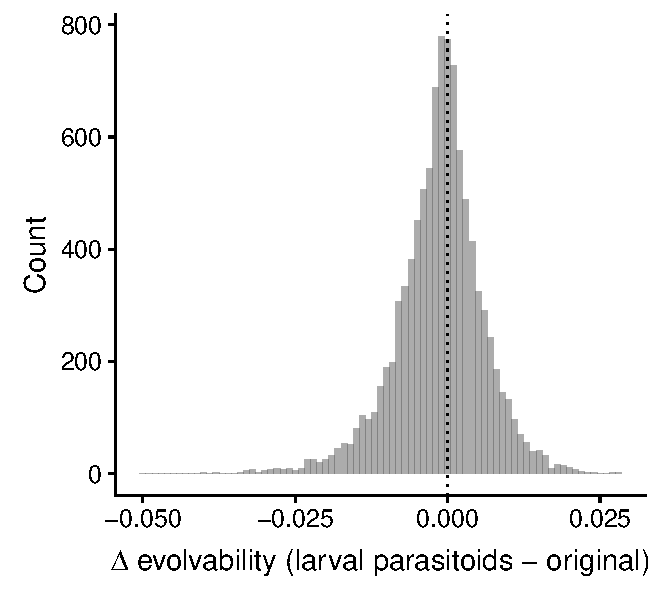
\includegraphics{../analyses/larvalptoid_delta_evolvability.pdf}
\caption{\label{fig:LarvalPtoidEvolvability}Change in average
evolvability for 10,000 random G-matrices using our best (mean) estimate
of the curvature matrix for selection in the absence of egg parasitoids
vs.~the original food web. We found that the curvature imposed by the
loss of egg parasitoids decreased evolvability in 57\% of the G-matrices
(i.e.~the change in evolvability was negative for 57\% of the
simulations), which is smaller in magnitude, but in the same direction,
as the effects of losing larval parasitoids.}
\end{figure}

\bibliography{references}


\end{document}
